\documentclass[9pt,twocolumn,twoside,lineno]{pnas-new}
% Use the lineno option to display guide line numbers if required.
% Note that the use of elements such as single-column equations
% may affect the guide line number alignment. 

\templatetype{pnasresearcharticle} % Choose template 
% {pnasresearcharticle} = Template for a two-column research article
% {pnasmathematics} = Template for a one-column mathematics article
% {pnasinvited} = Template for a PNAS invited submission

\title{Hack Weeks as a model for Data Science Education}

% Use letters for affiliations, numbers to show equal authorship (if applicable) and to indicate the corresponding author
\author[a,b,1]{Daniela Huppenkothen}
\author[c,d]{Anthony Arendt} 
\author[b,a,e,f]{David W. Hogg}
\author[g]{Karthik Ram}
\author[d]{Jake VanderPlas}
\author[d]{Ariel Rokem}

\affil[a]{Center for Data Science, New York University, 65 5th Avenue, 7th Floor, New York, NY 10003, USA}
\affil[b]{Center for Cosmology and Particle Physics, New York University, 726 Broadway, 10th Floor, New York, NY 10003, USA}
\affil[c]{Polar Science Center/Applied Physics Laboratory, University of Washington, 1013 NE 40th Street, Box 355640, Seattle, WA 98105-6698}
\affil[d]{The University of Washington eScience Institute, The WRF Data Science Studio, Physics/Astronomy Tower, 6th Floor, 3910 15th Ave NE, Campus Box 351570, University of Washington, Seattle, WA 98105, USA}
\affil[e]{Max-Planck-Institut f\"ur Astronomie, K\"onigstuhl 17, D-69117 Heidelberg}
\affil[f]{Center for Computational Astrophysics, Flatiron Institute, 162 5th Ave, New York, NY 10010, USA}
\affil[g]{Berkeley Institute for Data Science \& Berkeley Initiative in Global Change Biology, University of California, Berkeley,  Berkeley CA 94720}

% Please give the surname of the lead author for the running footer
\leadauthor{Huppenkothen} 

% Please add here a significance statement to explain the relevance of your work
\significancestatement{As scientific disciplines grapple with more data sets of rapidly increasing complexity and size, new approaches are urgently required to introduce new statistical and computational tools into research communities and improve the cross-disciplinary exchange of ideas. In this paper, we introduce a new type of scientific workshop, called a \textit{hack week}, which allows for fast dissemination of new methodologies into scientific communities, and fosters exchange and collaboration within and between disciplines. We present implementations of this concept in astronomy, neuroscience and geoscience, and show that hack weeks produce positive learning outcomes, foster lasting collaborations, yield scientific results and improve attitudes toward open science and reproducibility.}

% Please include corresponding author, author contribution and author declaration information
\authorcontributions{The concept was designed by Jake VanderPlas, the paper design initially by David W. Hogg, Karthik Ram and Jake VanderPlas. Daniela Huppenkothen, Ariel Rokem and Anthony Arendt performed the studies and the data analysis. All authors contributed to the final manuscript.}

\authordeclaration{The authors declare no conflicts of interest.}
%\equalauthors{\textsuperscript{1}A.O.(Author One) and A.T. (Author Two) contributed equally to this work (remove if not applicable).}
\correspondingauthor{\textsuperscript{1}To whom correspondence should be addressed. E-mail: daniela.huppenkothen@nyu.edu}

% Keywords are not mandatory, but authors are strongly encouraged to provide them. If provided, please include two to five keywords, separated by the pipe symbol, e.g:
\keywords{Data science $|$ Education $|$ Reproducibility $|$ Interdisciplinary Collaboration $|$ Astronomy $|$ Neuroscience $|$ Geosciences} 

%\begin{abstract}
%Please provide an abstract of no more than 250 words in a single paragraph. Abstracts should explain to the general reader the major contributions of the article. References in the abstract must be cited in full within the abstract itself and cited in the text.
%\end{abstract}
\begin{abstract}
Across almost all scientific disciplines, the instruments that record our experimental data and the methods required for storage and data analysis are rapidly increasing in complexity.
This gives rise to the need for scientific communities to adapt on shorter time scales than traditional university curricula allow for, and therefore requires new modes of knowledge transfer.
At the same time, as disciplines become more specialized, data analysis problems often tend to be fairly universal.
It is thus desirable to foster exchange of ideas and computational workflows across disciplines.
Among the different approaches put forward toward addressing these issues, hack weeks have in recent years emerged as both an effective tool for training researchers in modern data analysis workflows, and in fostering exchange between subdisciplines within and between scientific fields.
While interpreted differently in the various disciplines where they have been implemented, all events consist of a common core of three components: tutorials in state-of-the-art methodology, peer-learning and free-form project work.
In this paper, we present the concept of a hack week in the larger context of scientific meetings and point out similarities and differences to traditional conferences.
We motivate the need for such an event and present in detail its strengths and challenges.
We find that hack weeks are successful at cultivating collaboration and the exchange of knowledge.
Participants self-report that these events help them both in their day-to-day research as well as their careers.
Based on our results, we conclude that hack weeks present an effective, easy-to-implement, fairly low-cost tool to positively impact data analysis literacy in academic disciplines, foster collaboration and cultivate best practices.
\end{abstract}



\dates{This manuscript was compiled on \today}
\doi{\url{www.pnas.org/cgi/doi/10.1073/pnas.XXXXXXXXXX}}

\begin{document}


% Optional adjustment to line up main text (after abstract) of first page with line numbers, when using both lineno and twocolumn options.
% You should only change this length when you've finalised the article contents.
\verticaladjustment{-2pt}

\maketitle
\thispagestyle{firststyle}
\ifthenelse{\boolean{shortarticle}}{\ifthenelse{\boolean{singlecolumn}}{\abscontentformatted}{\abscontent}}{}

\section*{Introduction}
\label{sec:introduction}

As data becomes cheaper to gather and store, research across a wide range of disciplines has become increasingly reliant on computational workflows involving a familiarity with aspects of statistical modeling, machine learning, scalable computation, and related skills. In addition, the recent reproducibility crises in several scientific fields [REF] has led to the growing realization that improving awareness of open science and reproducibility as well as practical skills in making research reproducible is essential to scientific progress \cite[e.g.][]{pashler2012,frye2015,gezelter2015,baker2016}.
Formal university curricula have been relatively slow to offer courses in these important topics: the slack in this area has often been picked-up by extra-curricular, ad-hoc efforts such as workshops (an overview and typography of such efforts in the data science context can be found in \cite{demasi2017}).
Well-known examples are the Software and Data Carpentry workshops providing training in research computing skills through a volunteer instructor program  \cite{b:wilson-swc-lessons-2016,teal2015data}.
At the same time, there has been a rise in the number of domain-specific courses focusing on statistics and computation within their field.
Examples include the \textit{Summer School in Statistics for Astronomers}\footnote{\url{http://astrostatistics.psu.edu/su16/}}, the Google Earth Engine User Summits\footnote{\url{https://events.withgoogle.com/google-earth-engine-user-summit-2017/}}, as well as a variety of project-focused (rather than pedagogical) meetings, such as the dotAstronomy meetings\footnote{\url{http://dotastronomy.com}}.
Shorter, but similar-spirit meetings have been held in conjunction with conferences, such as the Hack Days at the annual American Astronomical Society meetings, the Brainhack hackathons that take place in conjunction with meetings of the Organization for Human Brain Mapping and the Society for Neuroscience\cite{Cameron_Craddock2016-wc}, and a hackathon at the American Geophysical Union meeting\footnote{\url{http://onlinelibrary.wiley.com/doi/10.1002/2014EO480004/pdf}}.
Generally, pedagogically-focused events follow a classic academic model where novices learn new skills from experts, while project-focused workshops emphasize collaborative activities using existing skills.
A disadvantage of the pedagogical model is that it can tends to focus on a one-way flow of information from instructor to student, and can discount the potential contributions by students.
A disadvantage of the project model is the common perception that the week is designed for technical experts, which may discourage others from attending.
In 2014, we initiated an alternative model of ``Hack Weeks'' that try to fill the gaps between these models.
These are week-long events that combine pedagogy (often focused on statistical and computational techniques) together with time for hacks and creative projects, and with the goal of encouraging collaboration and learning among people at various stages of their career.

%\begin{figure}
%\begin{center}
%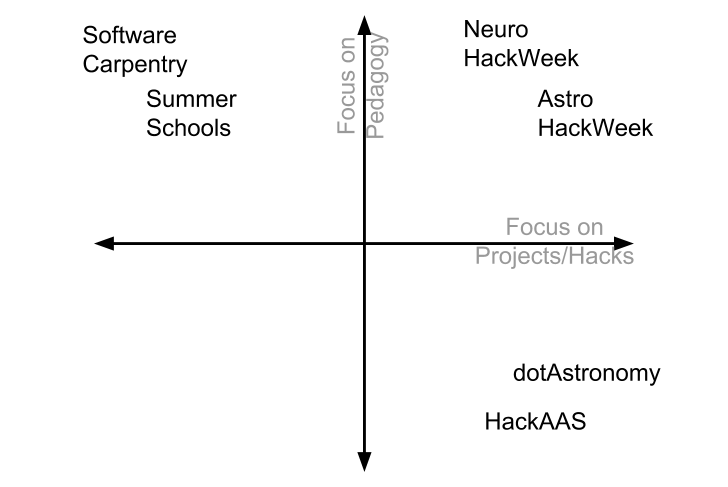
\includegraphics[width=9cm]{fig/HackSpectrum}
%\caption{Comparison of Extracurricular Workshop Models}
%\label{fig:hackspectrum}
%\end{center}
%\end{figure}

As of the publication of this paper, we have run eight such hack week events: four focused on Astronomy, two focused on Neuroscience, and two focused on Geoscience.
Below we will share some of the philosophy behind the hack week model, practical lessons we have learned in organizing these events, and recommendations for future hack weeks in other disciplines.

\section*{What is a hackathon?}

Hackathons are time-bounded, collaborative events that bring together participants around a shared challenge or learning objective \cite{Decker2015}.
Hackathons have historically focused on software development and technology design as a way to motivate innovation within industry.
In recent years, hackathons have expanded into a model for intensive short-term collaboration across disciplinary and topical boundaries.
In addition, because of their focus on participatory engagement, hackathons provide numerous opportunities to 'learn by doing' within a constructivist educational framework \cite{Bransford2000-lu,Papert1980-fh}.
With this in mind, hackathons around scientific topics, designed to foster collaboration \cite{Groen2015-cj,Moller2013-ah}, or provide an opportunity to learn \cite{Kienzler2015-zu,Lamers2014-xf}, are becoming more common.

%The recent surge in popularity of these events has resulted in a broad spectrum of ways to define the hackathon.
Following the typology of \cite{Drouhard2017}, we assert that core elements of all hackathons include opportunities for networking, the strengthening of social ties and the building of community connections, both within and across disciplines.
Building on these core elements, there are various implementations of the hackathon concept with respect to the overall purpose, mode of participation, style of work environment and motivation \cite{Drouhard2017}.
''Catalytic`` hackathons seek novel project ideas aimed at solving a tractable, well-defined challenge.
''Contributive`` hackathons seek to improve to an existing effort through focused work on discrete tasks, for example to make up for deficiencies in an ongoing project.
Finally, ''Communal`` hackathons place a strong focus on building a culture of practice and developing resources within an existing community, often defined by a specific domain of knowledge.

Our past hack week events most closely follow the communal hackathon model as it applies to scientific communities of practice.
Our approach aims to combine structured, tutorial-style instruction with informal education and peer learning opportunities occurring within projects and hacks.
Within the communal model we see these tools being implemented across a spectrum of approaches, the design of which depends on the specific characteristics of each community of practice (Figure 1).
For example, the astronomy community is relatively small and has a foundation of shared approaches and software implementations, allowing for a greater focus on project work over formal tutorials.
In contrast, both the neuro- and geoscience communities covered a broader range of sub-disciplines and had a less cohesive set of existing practices, calling for greater focus on tutorials and education.

We note that the terminology for these events is constantly evolving, and that the ''hackathon`` concept may have implicit connotations that are disfavored in some communities.
One criticism of hackathons is that they propel the ''geek`` stereotype and may present a barrier to creating an inclusive working environment, especially for women \cite{Decker2015}.
Another problem is the competitive atmosphere of many industry hackathons, where teams actively compete for prizes.
Because certain groups are more risk-averse than others, and risk-aversion traces demographics like gender, we urge caution when contemplating making an event competitive.
Other related nomenclature includes the ''unconference`` which is also a time-bounded event gathering together a specific community, but these often have minimal structure and do not necessarily have a focus on software.
The ''sprint`` or ''scrum`` label typically refers to an event focused on rapid software development on a specific set of code.
%This may be a component of our hack week model but it ignores the important pedagogical components.

\section*{Why run a Hack Week?}

There are several reasons to run a hack week of the sort described here.

\begin{itemize}
\item{\textit{Education and Training}: %Some hack weeks are more focused on education than others (see Figure 1).
While some hack weeks are focused more on education than others (Figure 1), there is often a skill-development component that entails extensive discussion on reproducible research and open science practices. Participants gain a strong foundation in open science practices from the diverse group setting and go on the become ambassadors for such practices in their respective fields. This type of lateral knowledge transfer is a core attribute of a hack week, and provides an opportunity to learn skills that are not described in papers and software implementations.}

\item{\textit{Tool Development}: Hack weeks present an opportunity for scientific software developers to meaningfully engage with users and critically evaluate applications to particular scientific issues.}

\item{\textit{Community Building}: Hack weeks provide a tremendous opportunity to catalyze community development through a shared interest in solving computational challenges with open source software. These events allow computationally minded researchers to break from the isolation of their academic departments and build connections and spark new collaborations.}


\item{\textit{Interdisciplinary research}: Intensive, time-bounded collaborative events are an excellent opportunity to experiment with concepts, questions, and methods that span boundaries within and across disciplines. Despite the fact that such interdisciplinary experiments are highly impactful \cite{Hall2012-hi}, they are often discouraged in risk averse traditional academia \footnote{\url{https://www.ncbi.nlm.nih.gov/labs/articles/12970550} and \url{https://www.researchgate.net/publication/8126355_EDUCATION_Risks_and_Rewards_of_an_Interdisciplinary_Research_Path}}}.

\item{\textit{Recruitment and Networking}: Hack weeks are often a melting pot of participants from academia, government, and industry and provide numerous opportunities for networking. Close collaboration in diverse groups exposes skills that might be suitable for careers outside of one's narrow domain.}

\item{\textit{It's fun}: Hack weeks provide a respite from day-to-day research activities and provide a low-stress venue to learn new skills and attempt high-risk projects.}

\end{itemize}


It is worth noting that the reasons for participants to attend a hack week are as diverse as the goals that the organizing committee explicitly states.
This is largely a function of the diversity of the participants (see section below), and should be something that organizers design for.
Beginner participants may attend primarily to learn a new technique or method, while more experienced participants attend to gain more experience mentoring and teaching.
Some researchers may come with particular projects and collaborators in mind, while others come with a focus on learning and with no explicit plan for the project-based work.
%While it is very hard to design a workshop that is universally useful to all participants, in practice many researchers attend with the understanding that some components will be more congruent with their own goals than others, but also bring an open mind and a willingness to learn.
%In addition, the diversity of goals can effectively be a strength of the workshop, if the organizers can facilitate matching up participants with complementary goals.

\section*{Audience and Participant Selection}

A thoughtful robust, and effective participant selection procedure is of crucial importance to the success of a hack week and may require both careful engineering and an in-depth discussion among the organizers.
At conferences, researchers typically report recent results to the community and network with other scientists, largely from their discipline.
In contrast, traditional summer schools aim for senior researchers to transfer knowledge about a particular subject or field to novice researchers, primarily graduate students and early postdoctoral fellows.
Hack weeks differ from both of these in that knowledge transfer occurs across many levels of seniority and across disciplinary boundaries, as well as novelty of the topics discussed,ranging from established theory to new findings.
In addition, the content is primarily participant-driven, and much of it is generated during the event itself.
This mean that a successful hack week requires participants who are both interested in participation, and also feel comfortable participating in discussions and taking risks.
Participant selection also addresses other objectives of a hack week such as increasing minority participation and gender diversity, knowledge transfer between academia and industry, etc. These factors can also be addressed by thoughtful participant selection.
To meet these goals, a thoughtful participant selection process needs to be as transparent to the applicants as possible, and the organizing committee should be held accountable for their performance in selecting participants.
Transparency is necessary for applicants to understand acceptance/rejection decisions, and accountability is of crucial importance for the detection of inherent biases in the selection, which may harm both the event's success as well as the larger community.
One way to maximize transparency in the selection process is to remove the human element from the decision making as far as possible and transfer some of these tasks to a well-designed algorithm.
In this context, well-designed means \cite{o2017weapons}: (1) interpretable, i.e. the algorithm, its parameters and outputs can be understood by humans, (2) openly available, and thus the decision process can be inspected, (3) the algorithm itself does not perpetuate intrinsic biases in the data (though we will show below that an algorithm itself does not entirely remove the requirement of humans to be aware of their biases).
In practice, most selection procedures follow two separate steps. In the first step, the merit of a candidate must be assessed: does the candidate fulfill the requirements posed by the goals of the workshop?
This first step is difficult to automate, because it requires judgment calls, often based on long-form answers.
To avoid implicit/unconcsious bias, in the past, we have sometimes performed this step by blinding ourselves to a candidate's other attributes (including name and other personal information), and assess their candidacy based solely upon key questions asked specifically for this purpose.
When doing this procedure for a large enough sample, it is unlikely that the resulting pool of acceptable candidates is smaller than the number of available spaces at the workshop.
The second step in the selection procedure then requires tie-breaking between equally acceptable candidates.
It is here where one may impose outside constraints on the selection based on the goals of the workshop.
If multiple competing constraints are considered, this task essentially becomes a complex optimization problem, for which algorithms exist that will outperform any human selection procedure.

On solution to this optimization procedure is implemented in the software \textit{entrofy}\footnote{\url{http://github.com/dhuppenkothen/entrofy}}. The algorithm maximizes the variance of participants on specified dimensions (e.g., career stage, geographic location, etc.) to meet pre-set fractions set by the organizers.
It is worth noting that this algorithm is vulnerable toward biases in two ways: firstly, humans will set the target fractions for any category of interest.
If these targets reproduce the distribution of the overall sample of candidates, the selection will become essentially random.
Any human biases involved in setting these target fractions will be perpetuated in the selection procedure.
Secondly, perhaps more obviously, the algorithm can only act on information that has been collected.
Biased participant sets may still result from selection procedures that fail to include crucial categories. For example, it would be difficult to produce a student-heavy participant set for a summer school if the algorithm has no information about academic seniority, and impossible to correct gender bias in the pool of applicants, if no information is available about the gender of participants.

\section*{Themes}

To date, all organized hack weeks have been subject-specific, i.e.\ aimed at bringing together a community with a shared scientific interest, such as neuroscience.
Advantages to this approach include shared language and scientific objectives within communities organized by subject, leaving more time for active collaboration on cutting-edge science.
On the other hand, homogeneity may lead to \textit{group think} and inhibit new, creative solutions. 
In this case, it may be advantageous to design a hack week around a technique (e.g.\ Gaussian Processes) or modality (e.g.\ imaging), such as the ImageXD (image processing across domains\footnote{\url{http://http://www.imagexd.org/}} meetings. 
For these events, building a shared vocabulary and understanding of major data analysis problems is crucial, but they also allow for cross-disciplinary diffusion of techniques into other subjects and therefore decrease the risk of duplication of method development efforts.

%This has several clear advantages.
%In particular, communities organized by subject generally share the same language.%, which drastically cuts down on the time participants spend simply agreeing on scientific terms.
%Similarly, the scientific objectives and questions are broadly clear to all participants.%: there is little need to explain in detail why a particular question may be of interest to the field.
%Finally, there are practical considerations: while even within fields the use of particular data sets and software packages may differ quite widely, there is generally a shared understanding of the type of data usually taken, and the most common ways to analyze this data.
%This leaves more time for active collaboration on cutting-edge science.

%However, there are also drawbacks to limiting the theme of a hack week to a single field.
%Homogeneity may be a disadvantage if it leads to \textit{group think} and inhibits new, creative solutions.
%Within a field, the chance of participants being familiar with each other may be larger, leading to the formation of cliques and insufficient mixing.
%These disadvantages may be mitigated by organizing a hack week around a technique (e.g. Gaussian Processes) or modality (e.g. imaging) instead.
%In these case, building a shared vocabulary and understanding the major data analysis problems in each field is a crucial task.%, and should be allocated sufficient time in form of introductory talks or tutorials to foster cross-disciplinary collaboration.
%On the other hand, cross-disciplinary hack weeks around a specific technique or type of data set allow methods developed in a specific field to diffuse into other subjects and therefore help avoid duplication of method development efforts.

%An example of such events are the ImageXD (image processing across domains\footnote{\url{http://http://www.imagexd.org/}} meetings held at the UC Berkeley Institute for Data Science in the Summer 2016, and at the UW eScience Institute in the Spring of %2017.
%These three-day events also included a mix of tutorials, talks, and joint work on projects, but in contrast to the hack weeks described in the present paper, these events included participants from a variety of different research fields, with the common thread being that they all have an interest in the analysis of images, as part their research.
%Thus, audience and speakers included researchers from wide array of domains: astronomy, neuroscience and geosciences, but also material science, chemistry, biology, medicine, engineering, and others.
%In addition, participants included computer vision researchers, who develop algorithms that can be applied to answer scientific questions.
%Similarly, a series of events at UC Berkeley (Text XD) focused on the analysis of text data across different domains of research.

\section*{Design considerations}

Scheduling, group size and venue are important design considerations contributing to the success of a hack week.   
Longer events allow for a larger taught component, more ambitious projects and cross-disciplinary exchanges. 
By spending more time together, participants are more likely to overcome barriers of professional terminology.
However, events that are too long may lead to fatigue among attendees, resulting in a drop in positive outcomes later in the workshop.
A well-designed hack week will have a clear schedule that limits the number of parallel sessions, in order to avoid decision fatigue, and will balance the duration of taught components and project work. 

A hackweek requires a flexible workspace environment with ample opportunity for re-configuration. 
Participants must have access to rooms that can accommodate lectures combined with interactive exchanges and individual work on laptops. 
Workspaces must also accommodate interactive project work where small teams can gather and work together.    
%Universities are an obvious first choice for hosting a hack week given their access to scientific resources, research support and infrastructure. 
%However traditional university lecture halls often do not meet the hack week criteria for interactive exchanges.
Fortunately, many universities are experimenting with other types of spaces: for example, the adoption of active learning teaching methods \cite{prince2004} has led to the development of modular classrooms, designed for group activities and flexible seating arrangements.

Another important design consideration is group size.
If the group is too large, chances for random participant exchanges are reduced, and knowledge transfer may decline as the workshop fractures into smaller groups, often among participants who already know each other.
If the group is too small, it is unlikely to achieve the desired level of diversity among participants to foster new collaborations across sub-fields and disciplines.
In the past, we have found groups with sizes between 50 and 70 participants to be large enough to encourage a breadth of projects while allowing the workshop to function as a cohesive group.

As mentioned above, the balance between pedagogy and open project work depends both on the goals of the workshop and the topics around which the workshop is organized.
If participants have little shared knowledge, more teaching may be necessary in order to allow participants to effectively communicate with each other.
In communities where a shared understanding exists, tutorials can be shortened to focus on more advanced or innovative topics, leaving more time for active participation.

Hack week outcomes depend strongly on the interest and engagement of participants.
Some attendees arrive with the goal of writing a scientific article, others plan to learn a specific topic, such as machine learning, or to analyze a specific data using the tools covered in the tutorials.
This leads to a wide variety of project types from sandbox-style explorations to focused work efforts.
This breadth of possible outcomes makes it difficult to design for all possible participant goals, and calls for adaptive, flexible leadership among hack week organizers.
The large variety in participant backgrounds and experiences--and the resulting range in personalities of attendees--requires careful, active facilitation of both taught and project components of a hack week. Community building is a core component of a hack week, and designs need to include both very strong personalities and very shy participants. In particular the presence of impostor syndrome experienced by many participants must be taken into account during workshop design (see also supplementary materials for concrete suggestions).
%can lead to an increase in the prevalence of impostor syndrome experienced by many participants (see also supplementary materials), and it 

\section*{Measures of success}

Measuring the success of a hack week objectively is complicated by the diversity of goals of both organizing committee and attendees.
A participant who attends primarily in order to hack on a specific project may find the tutorials less overall useful than a graduate student exposed to the tutorial topics for the first time.
Additionally, the participant-driven, open-ended format facilitates knowledge transfer and collaborations in sometimes surprising ways that escape traditional measures of success.
For more project-driven events, one key metric is the number of publications that result from hack week projects.
However, this implies a very narrow definition of success in line with standard academic performance indicators, and may be hard to collect in practice, if participants do not explicitly include a reference to the event in their publication.
Another, somewhat less traditional and complementary indicator is the activity of participants in terms of code written and committed to a public code repository (e.g. GitHub).
This could be defined in lines of code committed, the number of new open-source projects spawned, and the number of new developers contributing to open-source projects.
This assumes that participants work largely in the open during a hack week, and that most projects have a strong programming component.
Again, this may not be true for some hacks (e.g. tutorials, other written text, visualizations), and focuses entirely on material outcomes.
These measures ignore learning, community building as well as networking outcomes, which are often equally important objectives.
One possible approach here is to ask participants to self-report their success via a post-workshop survey.
It is in principle possible to measure gains in knowledge, networks and productivity within the pool of acceptable candidates for both those that attended the hack week and those that did not.
%This would then provide a somewhat objective measure of the impact the hack week has had.
%In practice, this has not been done for any of the hack weeks conducted thus far.
For practical purposes, we recommend an approach that combines all of these metrics: publications, new code and projects generated, self-reported learning outcomes, and survey results.
%Open-ended questions allow participants to provide feedback about outcomes, problems and goals that organizers had not anticipated.

If hack week organizers plan to conduct research that involves hack week participants (for example, using assessments and evaluations in a paper such as this one) it is important to obtain approval from the Institutional Review Board (IRB), or equivalent body that approves research with human participants at the institution hosting the hack week.
Though this research would usually fall under the category of ''minimal risk``, it is still important to establish procedures to manage these data, and to obtain informed consent.
In particular, in some cases hack week organizers may be interested in studying not only the participants in the hack week, but also the applicants who did not end up participating.
%It is important to establish procedures to conduct such studies and to obtain approval from an IRB.

\section*{Results}

In the following we report outcomes of previous events held in 2016 in three different fields (neuroscience, geoscience and astrophysics) and participants attitudes towards open science and reproducibility, their own learning outcomes, as well as community building and collaborations.
Because all three events are less than a year in the past, evaluating long-term outcomes (number of publications, citations, career outcomes) will require a longer baseline.
There are, however, initial indicators that all hack weeks encouraged long-term engagement with new concepts or tools and directly resulted in a number of publications \citep{gullysantiago2015,faria2016,keshavan2017,leonard2017,jordan2017,peterson2017,hahn2017,pricewhelan2017}.
[NOTE: HERE IS WHERE WE SHOULD REFER TO THE BOXES ONCE THEY ARE MERGED.]
We asked participants of all three hack weeks to complete surveys to validate the hack week's success.
%All surveys included a number of questions allowing participants to self-report their attitudes about the hack week in general as well as questions specifically designed to probe outcomes directly related to the hack week goals.

We find that at all three hack weeks, participant self-report successful learning outcomes in new topics, tools or methods (AHW: 86\%, GHW: 94\%, NHW: 76\% for responses ''somewhat agree``, ''agree`` and ''strongly agree``; Figure 2, left panel).
The overwhelming majority of respondents at the hack weeks ($>95\%$ for all three events) believed that they learned things that improve their day-to-day research, and that attendance has made them a better scientist (see Figure 2, middle and right panels).
%While each hack week also probed participants' attitudes in more detail toward specific topics, methods, and modes of learning, the hack weeks differed substantially on that level, making the results difficult to compare.
%Another important goal of the hack weeks was centred on community building and fostering collaborations.
We find that overall, the majority of participants felt that their contributions to their hack teams was valued, and that they built valuable connections to other researchers (Figure 3, middle panel).
This is especially true for Neuro Hack Week, where more than 64\% of participants strongly agreed that they formed valuable connections at NHW (Figure 3, right panel).
Because peer learning is a major mode of knowledge transfer at hack weeks, we asked participants whether they taught other participants.
We find that again a majority agrees with this statement to some degree (AHW: 83\%, GHW: 69\%, NHW: 71\% for combined responses ''somewhat agree``, ''agree`` and ''strongly agree``; Figure 3, left panel), though responses are not as unequivocal as they are in some of the other categories.
This is expected: participants new to the field may participate to learn rather than to teach.

Reproducibility and open science have recently drawn much attention from the scientific community, and all three hack weeks have been working to promote positive attitudes towards reproducibility and open science in their respective fields.
We find that hack weeks have been largely successful at encouraging open science: at all three events, more than 70\% of all participants (AHW: 79\%, GHW: 72\%, NHW:85\%; Figure 4, left panel) put code or data created at the hack week into a public repository, while a substantially smaller fraction of participants followed this practice before the event (Figure 4, middle panel).
When asking participants whether they had made their code or data openly available in the past, the overall behaviour reflects how general conventions and attitudes differ in different fields.
In particular, astronomy shows the largest degree of openness toward open science, whereas our results indicate that open science is still fairly uncommon in the geosciences, with neuroscience falling in between.
%Neuroscience seems to fall somewhere in between.
This implies that hack weeks can have the highest impacts in field where a priori engagement in reproducibility efforts is low and significant progress can be made towards changing researchers' attitudes during a collaborative workshop.
Similar attitudes are reflected when asking whether the hack week has made participants more comfortable with open science: again, geoscience shows the large improvement with over 97\% agreeing with this statement to some degree, closely followed by neuroscience (95\%), while there was somewhat less of an impact on participants' attitudes in astronomy (72\%).
Overall, our results show that hack weeks are effective at addressing persisting doubts about making research open and reproducible.
\begin{figure*}[htbp]
\begin{center}
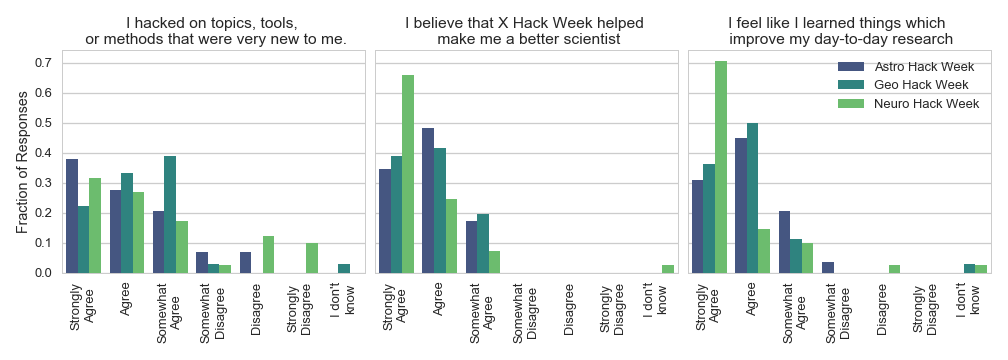
\includegraphics[\textwidth]{fig/eval_techskills.png}
\caption{Self-reported technical learning outcomes at all three hack weeks}
\label{fig:techskills}
\end{center}
\end{figure*}

\begin{figure*}[htbp]
\begin{center}
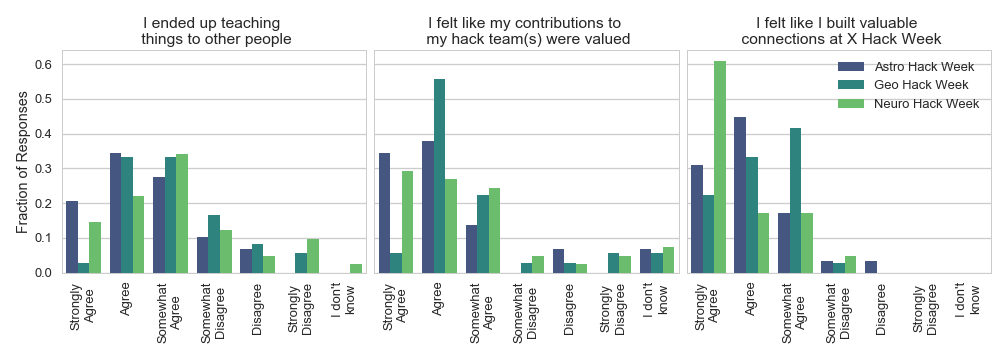
\includegraphics[\textwidth]{fig/eval_collab.png}
\caption{Hack week outcomes with respect to collaboration and peer-learning}
\label{fig:techskills}
\end{center}
\end{figure*}

\begin{figure*}[htbp]
\begin{center}
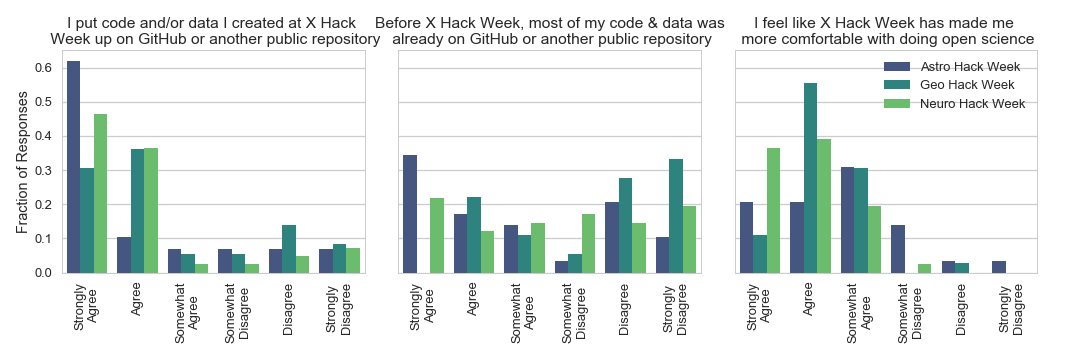
\includegraphics[\textwidth]{fig/eval_openscience.png}
\caption{Changing attitudes towards open science at hack weeks}
\label{fig:techskills}
\end{center}
\end{figure*}

\subsection*{Box 2: Examples of Hack Week Outcomes}
\subsubsection*{Example 1: Astro Hack Week}
In 2015, a small team used the opportunity of Astro Hack Week to found a new software project called Stingray\footnote{https://github.com/StingraySoftware/stingray} with the goal of providing well-tested, well-documented implementations of algorithms for time series analysis often used in X-ray astronomy.
The start of this project was facilitated by the collaborative environment at Astro Hack Week, including expertise in how to start/run open-source projects, role models of successful projects, and an environment encouraging scientific risk taking.
Since its beginnings at Astro Hack Week, Stingray has matured into an enduring collaboration within the community with five active maintainers, a number of contributors and four Google Summer of Code projects.
\subsubsection*{Example 2: Geo Hack Week}
In 2016, a Geo Hack Week project team used Google Earth Engine to explore spatial patterns in climate, topography and population data with the goal of mapping the most suitable locations for renewable energy sites in the United States.
The team used machine learning algorithms in conjunction with the powerful hardware resources provided by Google Earth Engine\footnote{\url{http://georgerichardson.net/2017/04/10/searching-for-energy-in-a-random-forest/}}.
George Richardson, one of the project leads, now works for a renewable resource company in Seattle.
\subsubsection*{Example 3: Neuro Hack Week}
Motion of study participants inside of the MRI machine is a major concern in neuroimaging studies.
This is a particular concern in studies in which children or patients are studied, as they are more likely to move.
In the 2016 Neuro Hack Week one of the teams focused on a large and openly available data-set of MRI data from children\footnote{ABIDE: \url{http://preprocessed-connectomes-project.org/abide}}.
To test the effect of motion on the results, the team conducted an analysis in which both the number of experimental subjects included, as well as motion cut-off were varied.
They tested both the split-half reliability of an analysis of brain connectivity, as well as an analysis that used machine learning to distinguish between brains of children with and without autism spectrum disorder.
The team (composed of four different researchers from four different institutions in two different countries) continued to work on this project remotely after the Neuro Hack Week was over, and they eventually wrote and published a paper describing these results in the open access journal Research Ideas and Outcomes \citep{leonard2017}.


\section*{Conclusions}

The fast-paced changes of the computational and methodological landscape require traditional fields of science to rapidly adapt to new data analysis challenges.
Traditional modes of learning, including university curricula, are often too slow to incorporate new developments on short enough time scales to meet their acute need in scientific advancement.
To address this imbalance, new types of workshops, including unconferences, hackathons and bootcamps, have been developed in recent years in various scientific disciplines to exist alongside with and support the existing structure of academic conferences.
Here, we introduce one such concept, hack weeks, and detail the underlying philosophical ideas along with experiences from events held in three different fields

As introduced above, hack weeks serve multiple purposes, including dissemination of state-of-the-art technological advances through the scientific community, building collaborations between academic subdisciplines and fostering interdisciplinary research as well as  promoting open science and reproducibility.
Initial results from three events held in 2016 \textbf{and 2017} in three different fields (astronomy, geosciences and neurosciences) indicate that hack weeks succeed at all of these objectives, but that the measure of success is field-specific in that it depends to some degree on how much the concepts hack weeks promote were already adopted within the community.
Hack weeks are still a very young concept, and estimating the long-term impact of these events within the scientific communities they serve will require follow-up over multiple years to asses their effect on collaboration networks, career outcomes for early-career academics and adoption of new methods.
We have shown, however, that hack weeks provide an easy-to-implement, fairly low-cost method to introduce new technologies and methods into scientific fields on much shorter time scales than traditional teaching efforts can.
\textbf{While we focus here on hack weeks in scientific fields, the concept could be extended to other areas, and is more generally useful in any area (1) where useful tools can be learned in short tutorials, (2) where results and outcomes can be produced on the timescale of a few days, and (3) that would benefit from collaborative approaches that cross traditional boundaries. Such areas could include for example the social sciences, music and art.}


% If your first paragraph (i.e. with the \dropcap) contains a list environment (quote, quotation, theorem, definition, enumerate, itemize...), the line after the list may have some extra indentation. If this is the case, add \parshape=0 to the end of the list environment.
%\dropcap{T}his PNAS journal template is provided to help you write your work in the correct journal format.  Instructions for use are provided below.

%Note: please start your introduction without including the word ``Introduction'' as a section heading (except for math articles in the Physical Sciences section); this heading is implied in the first paragraphs. 

%\section*{Guide to using this template on Overleaf}

%Please note that whilst this template provides a preview of the typeset manuscript for submission, to help in this preparation, it will not necessarily be the final publication layout. For more detailed information please see the \href{http://www.pnas.org/site/authors/format.xhtml}{PNAS Information for Authors}.

%If you have a question while using this template on Overleaf, please use the help menu (``?'') on the top bar to search for \href{https://www.overleaf.com/help}{help and tutorials}. You can also \href{https://www.overleaf.com/contact}{contact the Overleaf support team} at any time with specific questions about your manuscript or feedback on the template.

%\subsection*{Author Affiliations}

%Include department, institution, and complete address, with the ZIP/postal code, for each author. Use lower case letters to match authors with institutions, as shown in the example. Authors with an ORCID ID may supply this information at submission.

%\subsection*{Submitting Manuscripts}

%All authors must submit their articles at \href{http://www.pnascentral.org/cgi-bin/main.plex}{PNAScentral}. If you are using Overleaf to write your article, you can use the ``Submit to PNAS'' option in the top bar of the editor window. 

%\subsection*{Format}

%Many authors find it useful to organize their manuscripts with the following order of sections;  Title, Author Affiliation, Keywords, Abstract, Significance Statement, Results, Discussion, Materials and methods, Acknowledgments, and References. Other orders and headings are permitted.

%\subsection*{Manuscript Length}

%PNAS generally uses a two-column format averaging 67 characters, including spaces, per line. The maximum length of a Direct Submission research article is six pages and a PNAS PLUS research article is ten pages including all text, spaces, and the number of characters displaced by figures, tables, and equations.  When submitting tables, figures, and/or equations in addition to text, keep the text for your manuscript under 39,000 characters (including spaces) for Direct Submissions and 72,000 characters (including spaces) for PNAS PLUS.

%\subsection*{References}

%References should be cited in numerical order as they appear in text; this will be done automatically via bibtex, e.g. \cite{belkin2002using} and \cite{berard1994embedding,coifman2005geometric}. All references, including for the SI, should be included in the main manuscript file. References appearing in both sections should not be duplicated.  SI references included in tables should be included with the main reference section. 

%\subsection*{Data Archival}

%PNAS must be able to archive the data essential to a published article. Where such archiving is not possible, deposition of data in public databases, such as GenBank, ArrayExpress, Protein Data Bank, Unidata, and others outlined in the Information for Authors, is acceptable.

%\subsection*{Language-Editing Services}
%Prior to submission, authors who believe their manuscripts would benefit from professional editing are encouraged to use a language-editing service (see list at www.pnas.org/site/authors/language-editing.xhtml). PNAS does not take responsibility for or endorse these services, and their use has no bearing on acceptance of a manuscript for publication. 

%\begin{figure}%[tbhp]
%\centering
%\includegraphics[width=.8\linewidth]{frog}
%\caption{Placeholder image of a frog with a long example caption to show justification setting.}
%\label{fig:frog}
%\end{figure}

%\subsection*{Digital Figures}
%\label{sec:figures}

%Only TIFF, EPS, and high-resolution PDF for Mac or PC are allowed for figures that will appear in the main text, and images must be final size. Authors may submit U3D or PRC files for 3D images; these must be accompanied by 2D representations in TIFF, EPS, or high-resolution PDF format.  Color images must be in RGB (red, green, blue) mode. Include the font files for any text. 

%Figures and Tables should be labelled and referenced in the standard way using the \verb|\label{}| and \verb|\ref{}| commands.

%Figure \ref{fig:frog} shows an example of how to insert a column-wide figure. To insert a figure wider than one column, please use the \verb|\begin{figure*}...\end{figure*}| environment. Figures wider than one column should be sized to 11.4 cm or 17.8 cm wide.

%\subsection*{Single column equations}

%Authors may use 1- or 2-column equations in their article, according to their preference.

%To allow an equation to span both columns, options are to use the \verb|\begin{figure*}...\end{figure*}| environment mentioned above for figures, or to use the \verb|\begin{widetext}...\end{widetext}| environment as shown in equation \ref{eqn:example} below.

%Please note that this option may run into problems with floats and footnotes, as mentioned in the \href{http://texdoc.net/pkg/cuted}{cuted package documentation}. In the case of problems with footnotes, it may be possible to correct the situation using commands \verb|\footnotemark| and \verb|\footnotetext|.

%% Do not use widetext if paper is in single column.
%\begin{widetext}
%\begin{align*}
%(x+y)^3&=(x+y)(x+y)^2\\
%       &=(x+y)(x^2+2xy+y^2) \numberthis \label{eqn:example} \\
%       &=x^3+3x^2y+3xy^3+x^3. 
%\end{align*}
%\end{widetext}

%\begin{table}%[tbhp]
%\centering
%\caption{Comparison of the fitted potential energy surfaces and ab initio benchmark electronic energy calculations}
%\begin{tabular}{lrrr}
%Species & CBS & CV & G3 \\
%\midrule
%1. Acetaldehyde & 0.0 & 0.0 & 0.0 \\
%2. Vinyl alcohol & 9.1 & 9.6 & 13.5 \\
%3. Hydroxyethylidene & 50.8 & 51.2 & 54.0\\
%\bottomrule
%\end{tabular}

%\addtabletext{nomenclature for the TSs refers to the numbered species in the table.}
%\end{table}

%\subsection*{Supporting Information (SI)}

%The main text of the paper must stand on its own without the SI. Refer to SI in the manuscript at an appropriate point in the text. Number supporting figures and tables starting with S1, S2, etc. Authors are limited to no more than 10 SI files, not including movie files. Authors who place detailed materials and methods in SI must provide sufficient detail in the main text methods to enable a reader to follow the logic of the procedures and results and also must reference the online methods. If a paper is fundamentally a study of a new method or technique, then the methods must be described completely in the main text. Because PNAS edits SI and composes it into a single PDF, authors must provide the following file formats only.

%\subsubsection*{SI Text}

%Supply Word, RTF, or LaTeX files (LaTeX files must be accompanied by a PDF with the same file name for visual reference).

%\subsubsection*{SI Figures}

%Provide a brief legend for each supporting figure after the supporting text. Provide figure images in TIFF, EPS, high-resolution PDF, JPEG, or GIF format; figures may not be embedded in manuscript text. When saving TIFF files, use only LZW compression; do not use JPEG compression. Do not save figure numbers, legends, or author names as part of the image. Composite figures must be pre-assembled.

%\subsubsection*{3D Figures}

%Supply a composable U3D or PRC file so that it may be edited and composed. Authors may submit a PDF file but please note it will be published in raw format and will not be edited or composed.

%\subsubsection*{SI Tables}

%Supply Word, RTF, or LaTeX files (LaTeX files must be accompanied by a PDF with the same file name for visual reference); include only one table per file. Do not use tabs or spaces to separate columns in Word tables.

%\subsubsection*{SI Datasets} 

%Supply Excel (.xls), RTF, or PDF files. This file type will be published in raw format and will not be edited or composed. 

%\subsubsection*{SI Movies}

%Supply Audio Video Interleave (avi), Quicktime (mov), Windows Media (wmv), animated GIF (gif), or MPEG files and submit a brief legend for each movie in a Word or RTF file. All movies should be submitted at the desired reproduction size and length. Movies should be no more than 10 MB in size. 

%\subsubsection*{Still images}

%Authors must provide a still image from each video file. Supply TIFF, EPS, high-resolution PDF, JPEG, or GIF files. 

%\subsubsection*{Appendices}

%PNAS prefers that authors submit individual source files to ensure readability. If this is not possible, supply a single PDF file that contains all of the SI associated with the paper. This file type will be published in raw format and will not be edited or composed.

\matmethods{
We performed post-attendance survey for AstroHackWeek, GeoHackWeek and Neuro hack week in 2016. All three survey contained field-specific questions as well as general questions about attitudes towards the workshop as well as open science and reproducibility, and their own skills in statistical and computational methods. The latter set of questions were shared among all three surveys. All participants were e-mailed a personalized link to participate in the survey. The experimental procedures were approved by the Institutional Review Boards at UW, NYU and UC Berkeley. All participants gave their informed consent.
A total of X participants were e-mailed (AHW: 51, NHW: XX, GHW: XX) immediately after the survey, as well as XX weeks later. We received full responses from XX participants (AHW: 27, NHW: XX, GHW: XX), and partial responses from XX participants (AHW: 11, NHW: XX, GHW: XX). In this study, we predominantly focus on shared questions between all three surveys related to self-reported learning outcomes, collaboration and reproducibility. Participants were asked to respond to statements regarding these topics using a six-point Likert-type scale.


%\subsection*{Subsection for Method}
%Example text for subsection.
}

%\showmatmethods % Display the Materials and Methods section

\acknow{The authors would like to thank Laura Nor\'{e}n (NYU) for help on ethics and IRB, Stuart Geiger for helping to formulate the questionnaires that served as the basis for the results presented here, Brittany Fiore-Gartland, Laura Nor\'{e}n and Jason Yeatman for comments on the manuscript, and Tal Yarkoni for advice regarding automated selection procedures. This work was partially supported by the Moore-Sloan Data Science Environments at UC Berkeley, New York University, and the University of Washington. Neuro hack week is supported through a grant from the National Institute for Mental Health (1R25MH112480). Daniela Huppenkothen is partially supported by the James Arthur Postdoctoral Fellowship at NYU.}

\showacknow % Display the acknowledgments section

% \pnasbreak splits and balances the columns before the references.
% If you see unexpected formatting errors, try commenting out this line
% as it can run into problems with floats and footnotes on the final page.
\pnasbreak

% Bibliography
\bibliography{paper}

\end{document}